\section{Survey, Conduct, Design and Implement }

This chapter shows how the different iterations for this study were conducted. How the survey was made is explained, and how the decisions for criteria that should be used in the decision-model were made. It then talks about how the usability tests were performed and analyzed. Lastly, it goes through the evaluation and implementation of the decision-model.

\subsection{Conducting the survey}

The questions that were included in the mobile application discovery survey can be seen in table \ref{tab:survey-questions}.
\renewcommand{\arraystretch}{1.5}

\begin{table}[ht!]
    \centering
    \begin{tabularx}{0.9\textwidth} { 
        | >{\raggedright\arraybackslash}X 
        | >{\centering\arraybackslash}X 
        | >{\raggedleft\arraybackslash}X | }
        \hline
        How old are you? \\
        What type of smartphone do you primarily use? \\
        You just heard about a new smartphone application (app). Where do you turn when you want to find information about the app? \\
        You just heard about a new smartphone application (app). Where do you turn when you want to download the app? \\
        When you use the internet, how much time do you spend on apps versus web sites? \\
        How often do you think about your security and integrity when installing/downloading mobile applications? \\

        \hline
    \end{tabularx}
    \caption{\label{tab:survey-questions} Questions asked on the Internet usage survey.}
\end{table}

 The survey was implemented in Google Forms, and then distributed on the social media platform Facebook and posted on digital bulletin boards of The Royal Institute of Technology KTH in order to get as many responses as possible from different demographics. The survey was offered in both English and Swedish. After the data was collected, the answers were analyzed. This was done by comparison of how participants using Android answered versus how participants using iOS answered.

\subsection{Designing the decision model}

Since the model was to be used in the case of choosing a cross-platform implementation, only the options of developing either one PWA, two native applications or two applications using React Native were investigated. The two native platforms were Android, using the browser Google Chrome, and iOS, using the browser Safari.

\subsubsection{Deciding on criteria}

The criteria in the model were based on the literature study and brain-storming sessions with Slagkryssaren AB. During these sessions the business perspective, the developer perspective, the customer perspective and the end-user perspective were taken into account and discussed. The first set of criteria that were decided upon can be seen in table \ref{tab:first-criteria-version}. 


\begin{table}[ht]
    \centering
    \begin{tabular}{ |c|c| } 
        \hline
        Life span & Reachability \\
        \hline
          Micro transactions & Budget\\
          \hline
          Hardware support & Time-frame\\
          \hline
          Security & Customer skill set\\
          \hline
          Graphics & UX\\
        \hline
    \end{tabular}
    \caption{\label{tab:first-criteria-version} The first criteria selection.}
\end{table}

A few modifications were made to this list as the implementation progressed.

The criteria of \textit{Life-span} and \textit{Customer skill set} were later changed to be multiple-choice questions. These were hard to rank since the possible alternatives were few, for example the \textit{Life-span} as it was defined in this context could only have two possible outcomes: A permanent app or a temporary app. They also only affected the budget-aspect of the decision.

The criterion of \textit{Graphics} was partially combined with \textit{Hardware support} to form \textit{Performance}, and the remaining \textit{Hardware support} parts formed the new criterion \textit{Functions}.

\textit{Micro-transactions} was removed as a criterion, as the effect for each choice on the income for a micro-transaction business model was hard to define. The fee for using micro-transactions through App Store and Play Store was at the time of writing 30\%, which gives PWAs a benefit as a PWA bypasses the app stores \cite{IAPcost30}. Payment made in a PWA could be done on a multitude of payment services, but if a workaround like this was implemented, distributing an application through an app store becomes problematic. Also, for the end user there is an added convenience to purchasing applications and doing micro-transactions through an app store which were hard to quantify.

The criterion of \textit{Maintenance} was added to include the benefit of native applications from a maintenance and longevity standpoint, according to developers at Slagkryssaren AB.
\textit{Time-frame} was renamed \textit{Time to develop} to better define the criterion. 

The scores were decided based on discussion points from meetings with developers, literature studies, the statistically significant results from the UEQ, the first iteration of the qualitative data and the results from the mobile application discovery survey. The scores were set in relation to each other, meaning the best alternative on each criterion was given the score 10 and the other alternatives were given scores relative to this. The score for PWA and native application was set first, with the React Native being added afterwards.

Detailed reasoning for the scores were as follows:

\paragraph{Budget:} The Budget score was based on accounts from developers at Slagkryssaren AB. According to them it was approximately 30\% more expensive to develop a cross-platform solution than to develop one native application. This means developing two native applications was approximately 35\% more expensive than developing one PWA, and therefore the scores were set to 10 for PWA and 7 for native. React Native was given the score 9. This was based on the fact that up to 95\% of the code written is cross platform \cite{Ganguly2018}, and the rest is platform specific. It was therefore slightly more expensive than a PWA, but better than a native application. 

\paragraph{UX:} The UX score for the PWA was based on the usability test results. From the statistically significant results out of the UEQ, the PWA scored approximately 6:10 compared to the native application. The score for the React Native was based on information from developers at Slagkryssaren AB.

\paragraph{Functions:} The Functions score was intentionally set very low for PWA and high for the native application. If the decision-maker had many demands for functions not available on PWA, this would affect the weight, and if the decision-maker ranked the criterion Functions high it would give the native development method the desired advantage in that situation. Likewise, had the decision-maker few functions needed and/or no high ranking for the criterion, the weight would be very low, and so the scores could differ much without affecting the total outcome greatly. The most important feature for a PWA compared to a website on mobile was the offline mode and the home screen installation. Many functions were at the time of writing unavailable, so the PWA was given a score of 2 and native was given a 10. React Native was given a score of 9, based on the fact that almost all native functions can be accessed through a React Native application when using wrappers. 

\paragraph{Reachability:} The Reachability score was based on a number of factors. PWAs have an advantage in reachability, as they can be downloaded through most mobile browsers \cite{PWASupportingBrowsers}, and reached as websites without modifications through the others. PWAs could also be uploaded to Google Play store and, with some added difficulty, to Apples App store \cite{PWAonAppStore}. A PWA would also be available on desktop computers, laptops and tablets without the need to launch a separate website. The advantage of native applications in comparison is that there are at the time of writing less hoops to jump through to get your application on the app stores, and therefore they got a 5. React Native was estimated to have a similar reachability as native, but with the added benefit of having a Javascript-base allowing for easy translation into a website.

\paragraph{Maintenance:} According to developers at Slagkryssaren AB, native applications demand less maintenance as the environment is less volatile. In their experience, Javascript libraries and frameworks get deprecated or become outdated more frequently than code written in languages for native applications. This would mean a significantly larger workload to maintain the PWA, giving it a lower score than the native application. React Native has the dependencies of Javascript, combined with the added need for maintenance from OS updates, new device releases and two different platforms to handle debugging on. With this in mind, PWA was given 6, native 10 and React Native 4.

\paragraph{Time to develop:} The Time to develop score was based on information from developers at Slagkryssaren AB. Developing one PWA is much less time consuming than developing two native applications, and it can be launched through a browser without delay of app stores. React Native is slightly more time consuming than a PWA to launch, as it demands some extra code to be added to the Javascript-base to function on both platforms and for the applications to be approved on the app stores. Due to this, PWA was given the score 10, native application the score 5 and React Native application the score 7.

\paragraph{Performance:} The Performance score was based on literature studies and discussions with developers at Slagkryssaren AB. PWAs do not have the same direct link to the hardware of the unit as a native application does since they are run on a browser \cite[p.~12]{Yberg2018}, meaning the abstraction level is higher for a PWA than for a native application. This results in worse performance. 
This effect would, however, be preventable, as a PWA in some cases can be made to have almost native-like performance \cite[p.~43]{Yberg2018}. The React Native is a bit more complex to analyze. A well-implemented React Native application can have performance very similar to a native application \cite{Johansson2018}. However, according to Slagkryssaren AB a React Native application will on average be slightly worse than a native application, but not by as much as a PWA. With this in mind, the native application was given the score 10, the PWA the score 7 and the React Native application 8.5.

\subsubsection{Scoring and implementation}

The first version of the model was implemented with Google Spreadsheet. The input from the decision-maker was collected using Google Form.

In this version of the model the criteria and corresponding scores found in table  \ref{tab:model-score-v1} were set. 

\begin{table}[ht]
    \centering
    \begin{tabular}{ |c|c|c|c| } 
        \hline
        \rowcolor{light-gray}
        Criterion & PWA & Native & React \\
        \hline
        Budget & 10 & 7 & 9\\ 
        \hline
        UX & 6 & 10 & 8\\ 
        \hline
        Functions & 2 & 10 & 9\\ 
        \hline
        Reachability & 10 & 5 & 8\\
        \hline
        Maintenance & 6 & 10 & 4\\
        \hline
        Time to develop & 10 & 5 & 7\\
        \hline
        Performance & 7 & 10 & 8,5\\
        \hline
    \end{tabular}
    \caption{\label{tab:model-score-v1}Scores set for the first version of the model.}
\end{table}

The model used three types of input from the user.
Firstly, the user was presented with the functions which are currently unavailable for a PWA on iOS and/or Android. They were instructed to select the functions they needed for the application (see list in figure \ref{tab:model-func-unavail}). This affected the weight for the criteria \textit{Functions}, the more functions selected, the higher the weight. The effect was calculated by summation of the selected functions' corresponding number of unavailable platforms, dividing the sum by the total 20 and added by one. This produced a number between 1 and 2, depending on how many functions were selected. 
















\begin{table}[ht]
    \centering
    \begin{tabular}{ |c|c| }
        \hline
        \rowcolor{light-gray}
        Function & no. platforms unavailable\\
        \hline
        App store presence & 1 \\ 
        \hline
        Integrated camera function & 1 \\ 
        \hline
        Bluetooth & 1 \\ 
        \hline
        NFC & 2 \\
        \hline
        Notifications & 1 \\
        \hline
        Surrounding sensors $^1$  & 2 \\
        \hline
        Vibration & 1 \\
        \hline
        Contacts & 2 \\
        \hline
        Scheduling & 2 \\
        \hline
        Background sync & 1 \\
        \hline
        High accuracy GPS & 2 \\
        \hline
        Geofencing & 2 \\
        \hline
        VR/AR & 1 \\
        \hline
        Advanced screen manipulation $^2$  & 1 \\
        \hline 

    \end{tabular}
    \caption{\label{tab:model-func-unavail}Functions and how many platforms out of iOS and Android they remain unavailable on when choosing PWA. \\
    \textit{$^1$Surrounding sensors includes ambient light and proximity sensor}\\
    \textit{$^2$Advanced screen manipulation includes orientation, full screen and wake lock}
    } 
\end{table}

Second, a number of multiple-choice questions were asked.

\begin{itemize}
    \item \textit{Competences}: Which competencies are available in the customers business?
        \begin{itemize}
            \item Web: \textit{Multiply Budget with 1.5}
            \item Android and/or iOS: \textit{Multiply Budget with 0.5}
            \item All of the above: \textit{No effect}
            \item None of the above: \textit{No effect}
        \end{itemize}
    \item \textit{Website}: Does a website with the same functions already exist? 
        \begin{itemize}
            \item Yes: \textit{Multiply Budget with 1.3}
            \item No: \textit{No effect}
        \end{itemize}
    \item \textit{Short-lived}: Is the app short-lived?
        \begin{itemize}
            \item Yes: \textit{Multiply Maintenance with 0.5}
            \item No: \textit{No effect}
        \end{itemize}
\end{itemize}

These questions affected the weights of certain criteria. \textit{Competences} and \textit{Website} affected the criterion Budget. If the customer business had competences within web-programming, the weight was increased, as this gave further advantage to PWAs and React Native applications. Same with the website, a website can be converted to a PWA easily, and to a React Native application with slightly more work, which would save time and money. If the customer held competences in native application programming, the weight was decreased, as this made native applications less expensive in the long run compared to PWAs and React Native applications.

The question of \textit{Short-lived} affected the criterion of Maintenance. If the application was short-lived, the disadvantage of the higher demand for maintenance on a PWA and React Native application was lessened. The risk of a utilized function or library being deprecated would, however, still be present.

After that, the user ranked the criteria on importance. The criterion with the highest ranking was given the most weight, one to 100.
The last step of the process multiplied in the numbers given by the multiple-choice questions and the function-selection on the relevant criteria, and then normalized so that the weights summed to 1, according to WSM standards.  

\subsection{Conducting comparative usability tests}
The test subjects were recruited through a form shared on the social media platform Facebook and posted on bulletin boards at the campus of KTH. The test subjects were compensated with a goodie-bag and free coffee.
The first tests were conducted at the office of Slagkryssaren AB. The tests were later moved to the campus of The Royal Institute of Technology KTH.

The product chosen for the usability test was the recipe application Yummly. Yummly has both a native Android application and a native iOS application, and a PWA. Yummly was chosen for the test since it had a good amount of interaction elements, and it would be possible to put the test participants in realistic scenarios. The product itself was relatively intuitive and relateable for most people. Since the application was not developed for the Swedish market, it would be unlikely that the test participants had used the application before. Yummly had several interaction elements, some of which were included in the tests including searching, filtering and navigation of menus. An example of the differences in the views can be seen in figures \ref{fig:yummly_screenshot:1} and \ref{fig:yummly_screenshot:2}.

\begin{figure}[ht]
	\centering 
	\subfloat[Native iOS]{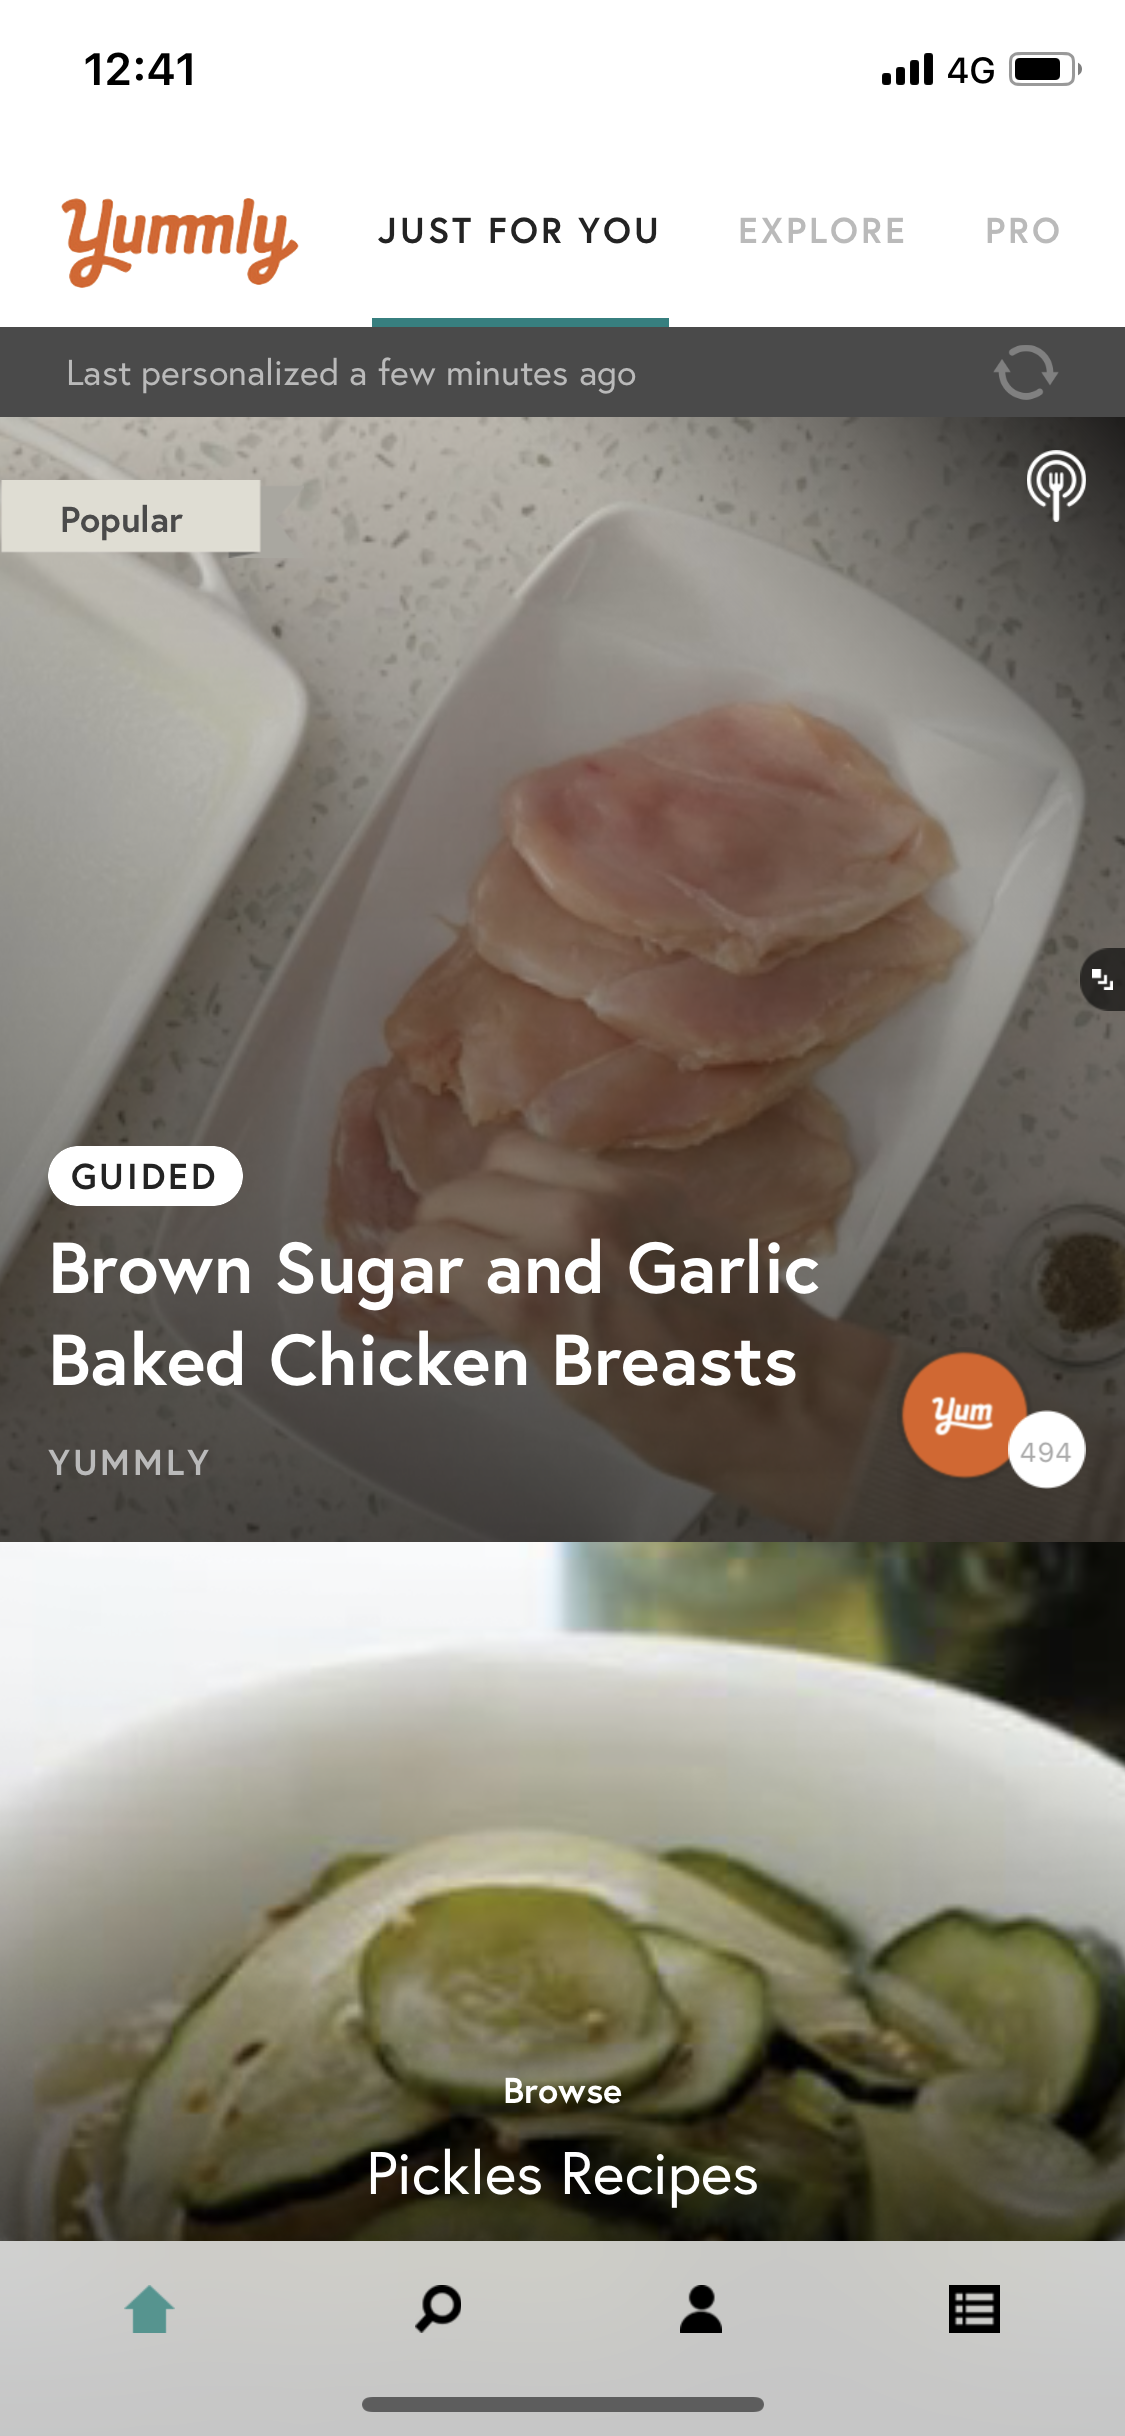
\includegraphics[width=0.3\textwidth]{img/yummly_screenshot_native.png}
		\label{fig:yummly_screenshot:1}}
	%\hfill
	\subfloat[PWA iOS]{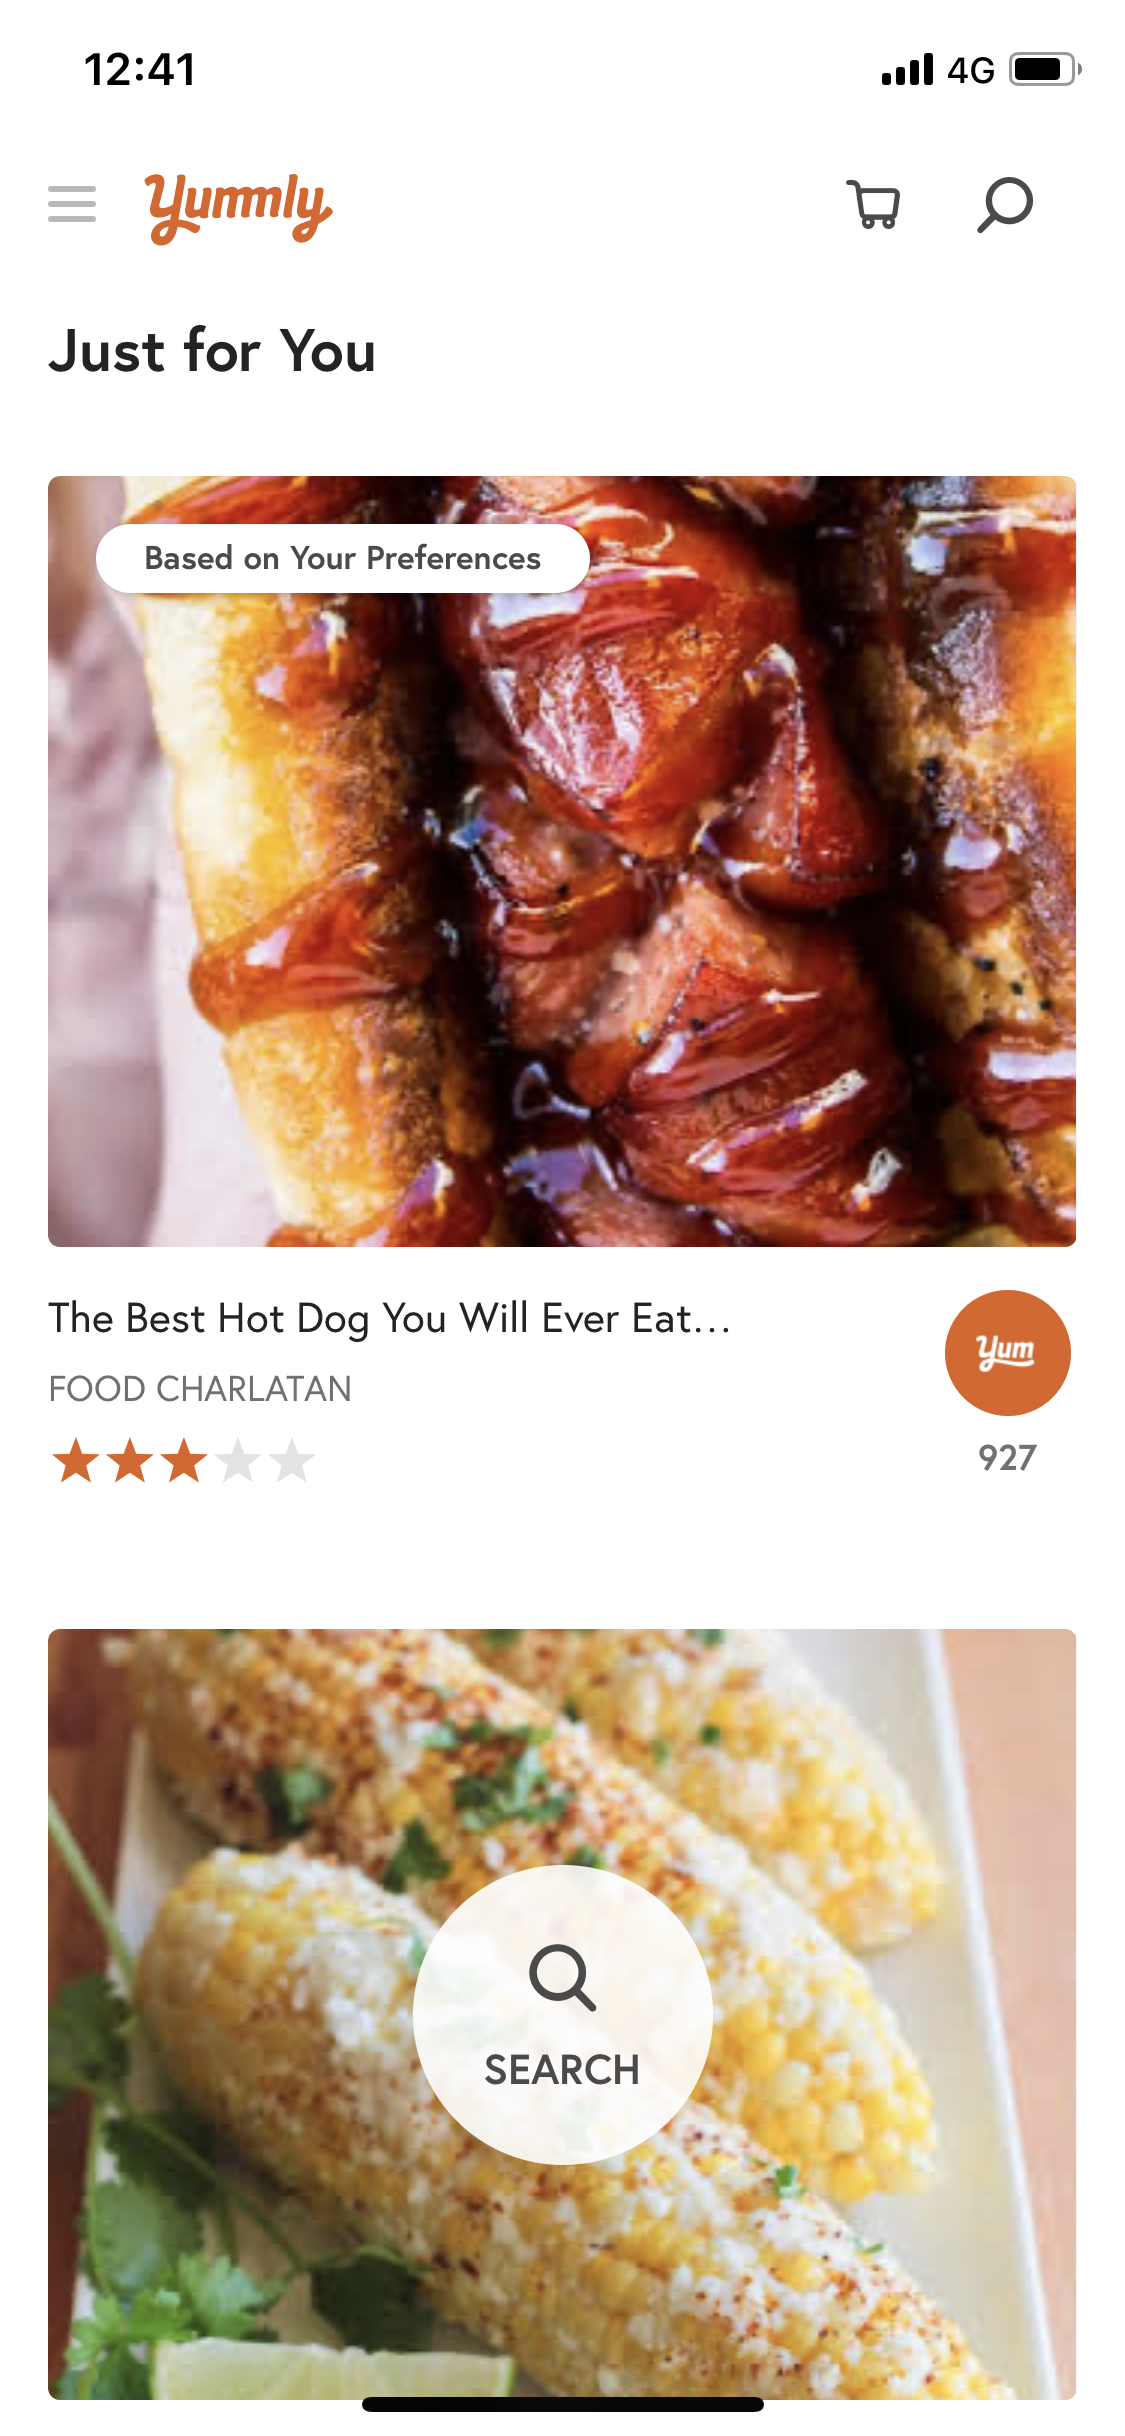
\includegraphics[width=0.3\textwidth]{img/yummly_screenshot_pwa.png}
		\label{fig:yummly_screenshot:2}}
	\caption{\textit{Screenshots of the different versions of the Yummly application.}}
	\label{fig:yummly_screenshots}
\end{figure}


Before each test, the subjects answered some background questions, shown in table  \ref{tab:background-questions}. These were used both to gather more information for the statistical review of the test results and to make the subjects more open and ready to talk. The subject also filled in a consent form. The consent form made it possible to record and process the recorded material for analysis of the qualitative data. The consent form can be read in appendix \ref{appendix:consent_forms}.

\begin{table}[ht!]
    \centering
    \begin{tabularx}{0.9\textwidth} { 
        | >{\raggedright\arraybackslash}X 
        | >{\centering\arraybackslash}X 
        | >{\raggedleft\arraybackslash}X | }
        \hline
        What is your main occupation? \\
        How much time do you spend on your smartphone on an average day? \\
        How much of that time do you spend on applications versus websites? \\
        What kind of mobile applications do you mostly use? Work, chat, social media, finances,  shopping etc.?\\
        \hline
    \end{tabularx}
    \caption{\label{tab:background-questions} Background questions for the usability tests.}
\end{table}

For the user tests, the Nielsen Norman Group’s article on task scenarios for usability tests was used \cite{NielsenTask2014}. The scenarios were designed to be relatively realistic, actionable and with an appropriate level of vagueness for the test subjects to have to think when they performed the tasks. The scenarios in table \ref{tab:usability-test-tasks} were included in the first tests.

\begin{table}[ht!]
    \centering
    \begin{tabularx}{0.9\textwidth} { 
        | >{\raggedright\arraybackslash}X 
        | >{\centering\arraybackslash}X 
        | >{\raggedleft\arraybackslash}X | }
        \hline
        1. Find the recipe “Avocado vegan fudge brownie” \\
        2. Use the app to find recipes with chicken which take less than 15 minutes to cook \\
        3. You are making dinner. Use the app to make a shopping list for: a dish with fish, a dish with bacon, and a dessert \\
        4. One can add their dietary preferences/allergies in the app. Try adding that you eat gluten-free and vegan, and find recipes for chilli. Browse around and find a recipe you find interesting. \\
        5. It’s possible to save recipes through a so-called “Yum’s” list. Create a “Yum’s” list called Pastries and add a few recipes to the list \\
        6. Add “milk” and “eggs” to the shopping list \\
        7. You’re in the store and have now picked up eggs, update your shopping list. \\
        \hline
    \end{tabularx}
    \caption{\label{tab:usability-test-tasks} The first list of tasks.}
\end{table}

The tests were recorded with a camera, showing the face and recording the voice of the test subject. This allowed for richer, more nuanced qualitative data to be gathered from the usability tests, and also allowed for tests to be revisited and analyzed a posteriori. This was useful since there were only two people conducting the tests, and neither has extensive experience in usability testing. After three tests, another camera was added, recording the subjects' from behind. This allowed the researchers to see what the subject was reacting to on the device.

Pilot tests were performed first to assess how well the thought out scenarios worked. The pilot tests were timed to evaluate how time-consuming the different parts of the test were. These pilot tests averaged at 30-40 minutes in total. Some scenarios were removed and edited to minimize time consumption, without affecting the quality of the results. The order of the tasks was also changed to better mimic how the application would be used in real life. Scenario number 6 was put first for this reason. Scenario number 1 was removed because scenario 2 and 4 filled the same function.

The SUS, UEQ and consent forms were initially printed on paper to ease the process of filling them in. Since the computer was used for facial recording, the subject was forced to lean over to reach the touch-pad. After the pilot tests, this was changed to have the subjects fill in the SUS and UEQ on the computer instead. This saved both time and the amount of paper used for the tests. The data from the SUS and UEQ was stored digitally to be used for statistics. The tests were saved separately depending on the device used and the type of application tested. This would ease the statistical analysis between the platforms. The aspect of Novelty from the UEQ was left out of this test, as it was not within the scope of the research question.

\subsection{Analyzing the usability tests}

The results from the SUS and the UEQ were compiled and then evaluated on the statistical significance of the data. 
The qualitative data recorded in text from the usability test was processed and compiled to form the first qualitative base for the test results.

\subsection{Evaluating the Decision-making model}

The first version of the model was tested by iteratively running scenarios through the model and evaluating the results. Some of these scenarios were constructed for the purpose of testing if the model gave reasonable results in "ideal" native application or PWA scenarios, and some scenarios were taken from real-life applications implemented either as native applications, React Native applications or PWAs.

After a few rounds of testing, the score for Functions was changed from 1 to 2 on PWA. The motivation for this was that even in the cases where few functions were chosen as necessary for the application, the native got a huge advantage in the score. Changing the score for PWA evened out the playing field a bit, without affecting the cases where native applications had a clear advantage. It also represents the available functionality better, a PWA is similar to a website on mobile devices but has some distinguishing functions such as offline mode and home-screen installation.

When the model seemed to be acting reasonably, a consultant from Slagkryssaren AB was invited to test the model out. The consultant noted that the model as it was implemented at the time seemed to give the accurate recommendation compared to how he provided input. The consultant's overall feedback of the model was positive, noting that it would be a useful tool for the earlier stages of the development process. It gave a good ground for discussion and could give the developing team another opportunity to consider what could be necessary for the project. At this point it was decided that the model was finished.
